\documentclass{standalone}
\usepackage{tikz}
\usetikzlibrary{patterns, positioning}

\begin{document}
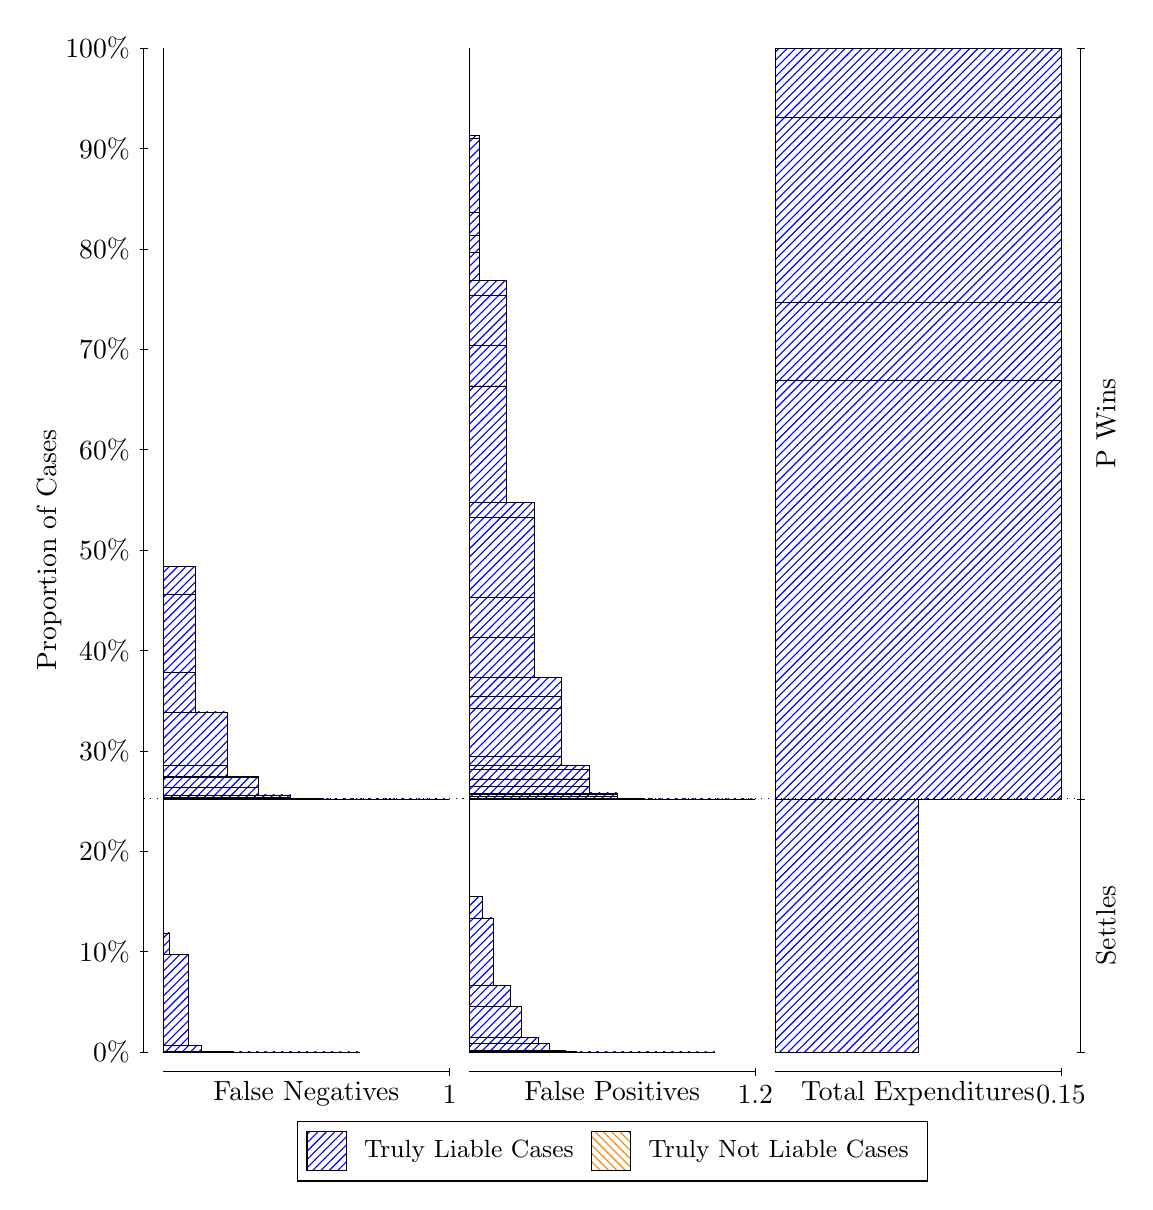
\begin{tikzpicture}
\draw[black, very thin] (1.5,1.75) -- (1.5,14.5);
\node[rotate=90, anchor=center] at (0.3, 8.125) {Proportion of Cases};
\draw[black, very thin] (1.45,1.75) -- (1.55,1.75);
\node[anchor=east] at (1.45, 1.75) {0\%};
\draw[black, very thin] (1.45,3.025) -- (1.55,3.025);
\node[anchor=east] at (1.45, 3.025) {10\%};
\draw[black, very thin] (1.45,4.3) -- (1.55,4.3);
\node[anchor=east] at (1.45, 4.3) {20\%};
\draw[black, very thin] (1.45,5.575) -- (1.55,5.575);
\node[anchor=east] at (1.45, 5.575) {30\%};
\draw[black, very thin] (1.45,6.85) -- (1.55,6.85);
\node[anchor=east] at (1.45, 6.85) {40\%};
\draw[black, very thin] (1.45,8.125) -- (1.55,8.125);
\node[anchor=east] at (1.45, 8.125) {50\%};
\draw[black, very thin] (1.45,9.4) -- (1.55,9.4);
\node[anchor=east] at (1.45, 9.4) {60\%};
\draw[black, very thin] (1.45,10.675) -- (1.55,10.675);
\node[anchor=east] at (1.45, 10.675) {70\%};
\draw[black, very thin] (1.45,11.95) -- (1.55,11.95);
\node[anchor=east] at (1.45, 11.95) {80\%};
\draw[black, very thin] (1.45,13.225) -- (1.55,13.225);
\node[anchor=east] at (1.45, 13.225) {90\%};
\draw[black, very thin] (1.45,14.5) -- (1.55,14.5);
\node[anchor=east] at (1.45, 14.5) {100\%};

\draw[black, very thin] (13.4,1.75) -- (13.4,14.5);
\draw[black, very thin] (13.35,1.75) -- (13.45,1.75);
\node[anchor=west] at (13.35, 1.75) {};
\draw[black, very thin] (13.35,4.9648) -- (13.45,4.9648);
\node[anchor=west] at (13.35, 4.9648) {};
\draw[black, very thin] (13.35,14.5) -- (13.45,14.5);
\node[anchor=west] at (13.35, 14.5) {};

\draw[black, very thin, pattern color=blue, pattern=north east lines] (1.75,1.75) rectangle (4.2479,1.75);
\draw[black, very thin, pattern color=blue, pattern=north east lines] (1.75,1.75) rectangle (3.8442,1.75);
\draw[black, very thin, pattern color=blue, pattern=north east lines] (1.75,1.75) rectangle (3.4405,1.75);
\draw[black, very thin, pattern color=blue, pattern=north east lines] (1.75,1.75) rectangle (3.1579,1.75);
\draw[black, very thin, pattern color=blue, pattern=north east lines] (1.75,1.75) rectangle (3.0368,1.7503);
\draw[black, very thin, pattern color=blue, pattern=north east lines] (1.75,1.7503) rectangle (2.7542,1.7503);
\draw[black, very thin, pattern color=blue, pattern=north east lines] (1.75,1.7503) rectangle (2.6331,1.7581);
\draw[black, very thin, pattern color=blue, pattern=north east lines] (1.75,1.7581) rectangle (2.3505,1.7581);
\draw[black, very thin, pattern color=blue, pattern=north east lines] (1.75,1.7581) rectangle (2.2294,1.8376);
\draw[black, very thin, pattern color=blue, pattern=north east lines] (1.75,1.8376) rectangle (2.0679,2.9894);
\draw[black, very thin, pattern color=blue, pattern=north east lines] (1.75,2.9894) rectangle (1.9468,2.9894);
\draw[black, very thin, pattern color=blue, pattern=north east lines] (1.75,2.9894) rectangle (1.8257,3.2613);
\draw[black, very thin, pattern color=orange, pattern=north west lines] (1.75,3.2613) rectangle (1.75,3.2613);
\draw[black, very thin, pattern color=blue, pattern=north east lines] (1.75,3.2613) rectangle (1.75,4.9648);
\draw[black, very thin, pattern color=blue, pattern=north east lines] (1.75,4.9648) rectangle (5.3833,4.9648);
\draw[black, very thin, pattern color=blue, pattern=north east lines] (1.75,4.9648) rectangle (4.9796,4.9648);
\draw[black, very thin, pattern color=blue, pattern=north east lines] (1.75,4.9648) rectangle (4.5759,4.9648);
\draw[black, very thin, pattern color=blue, pattern=north east lines] (1.75,4.9648) rectangle (4.5759,4.9648);
\draw[black, very thin, pattern color=blue, pattern=north east lines] (1.75,4.9648) rectangle (4.1722,4.965);
\draw[black, very thin, pattern color=blue, pattern=north east lines] (1.75,4.965) rectangle (4.1722,4.9652);
\draw[black, very thin, pattern color=blue, pattern=north east lines] (1.75,4.9652) rectangle (3.7685,4.9702);
\draw[black, very thin, pattern color=blue, pattern=north east lines] (1.75,4.9702) rectangle (3.3648,4.9887);
\draw[black, very thin, pattern color=blue, pattern=north east lines] (1.75,4.9887) rectangle (3.3648,5.0149);
\draw[black, very thin, pattern color=blue, pattern=north east lines] (1.75,5.0149) rectangle (2.9611,5.1056);
\draw[black, very thin, pattern color=blue, pattern=north east lines] (1.75,5.1056) rectangle (2.9611,5.2352);
\draw[black, very thin, pattern color=blue, pattern=north east lines] (1.75,5.2352) rectangle (2.9611,5.2542);
\draw[black, very thin, pattern color=blue, pattern=north east lines] (1.75,5.2542) rectangle (2.5574,5.394);
\draw[black, very thin, pattern color=blue, pattern=north east lines] (1.75,5.394) rectangle (2.5574,6.0694);
\draw[black, very thin, pattern color=blue, pattern=north east lines] (1.75,6.0694) rectangle (2.1537,6.5728);
\draw[black, very thin, pattern color=blue, pattern=north east lines] (1.75,6.5728) rectangle (2.1537,7.5587);
\draw[black, very thin, pattern color=blue, pattern=north east lines] (1.75,7.5587) rectangle (2.1537,7.9176);
\draw[black, very thin, pattern color=orange, pattern=north west lines] (1.75,7.9176) rectangle (1.75,7.9176);
\draw[black, very thin, pattern color=blue, pattern=north east lines] (1.75,7.9176) rectangle (1.75,14.5);
\draw[black, very thin, pattern color=orange, pattern=north west lines] (5.6333,1.75) rectangle (8.7533,1.75);
\draw[black, very thin, pattern color=blue, pattern=north east lines] (5.6333,1.75) rectangle (8.7533,1.75);
\draw[black, very thin, pattern color=blue, pattern=north east lines] (5.6333,1.75) rectangle (8.4022,1.75);
\draw[black, very thin, pattern color=blue, pattern=north east lines] (5.6333,1.75) rectangle (8.0512,1.75);
\draw[black, very thin, pattern color=orange, pattern=north west lines] (5.6333,1.75) rectangle (7.8054,1.75);
\draw[black, very thin, pattern color=blue, pattern=north east lines] (5.6333,1.75) rectangle (7.8054,1.75);
\draw[black, very thin, pattern color=blue, pattern=north east lines] (5.6333,1.75) rectangle (7.7001,1.75);
\draw[black, very thin, pattern color=blue, pattern=north east lines] (5.6333,1.75) rectangle (7.4544,1.75);
\draw[black, very thin, pattern color=blue, pattern=north east lines] (5.6333,1.75) rectangle (7.3491,1.7503);
\draw[black, very thin, pattern color=blue, pattern=north east lines] (5.6333,1.7503) rectangle (7.1033,1.7503);
\draw[black, very thin, pattern color=blue, pattern=north east lines] (5.6333,1.7503) rectangle (6.998,1.7581);
\draw[black, very thin, pattern color=orange, pattern=north west lines] (5.6333,1.7581) rectangle (6.8576,1.7581);
\draw[black, very thin, pattern color=blue, pattern=north east lines] (5.6333,1.7581) rectangle (6.8576,1.7695);
\draw[black, very thin, pattern color=blue, pattern=north east lines] (5.6333,1.7695) rectangle (6.7523,1.7695);
\draw[black, very thin, pattern color=blue, pattern=north east lines] (5.6333,1.7695) rectangle (6.647,1.8544);
\draw[black, very thin, pattern color=blue, pattern=north east lines] (5.6333,1.8544) rectangle (6.5066,1.9391);
\draw[black, very thin, pattern color=blue, pattern=north east lines] (5.6333,1.9391) rectangle (6.4012,1.9391);
\draw[black, very thin, pattern color=blue, pattern=north east lines] (5.6333,1.9391) rectangle (6.2959,2.327);
\draw[black, very thin, pattern color=blue, pattern=north east lines] (5.6333,2.327) rectangle (6.1555,2.5999);
\draw[black, very thin, pattern color=blue, pattern=north east lines] (5.6333,2.5999) rectangle (6.0502,2.6);
\draw[black, very thin, pattern color=blue, pattern=north east lines] (5.6333,2.6) rectangle (5.9449,3.4535);
\draw[black, very thin, pattern color=blue, pattern=north east lines] (5.6333,3.4535) rectangle (5.8045,3.7254);
\draw[black, very thin, pattern color=blue, pattern=north east lines] (5.6333,3.7254) rectangle (5.6992,3.7254);
\draw[black, very thin, pattern color=blue, pattern=north east lines] (5.6333,3.7254) rectangle (5.6333,4.9648);
\draw[black, very thin, pattern color=orange, pattern=north west lines] (5.6333,4.9648) rectangle (9.2667,4.9648);
\draw[black, very thin, pattern color=blue, pattern=north east lines] (5.6333,4.9648) rectangle (9.2667,4.9648);
\draw[black, very thin, pattern color=orange, pattern=north west lines] (5.6333,4.9648) rectangle (8.9156,4.9648);
\draw[black, very thin, pattern color=blue, pattern=north east lines] (5.6333,4.9648) rectangle (8.9156,4.9648);
\draw[black, very thin, pattern color=orange, pattern=north west lines] (5.6333,4.9648) rectangle (8.5646,4.9648);
\draw[black, very thin, pattern color=blue, pattern=north east lines] (5.6333,4.9648) rectangle (8.5646,4.9648);
\draw[black, very thin, pattern color=blue, pattern=north east lines] (5.6333,4.9648) rectangle (8.5646,4.9648);
\draw[black, very thin, pattern color=blue, pattern=north east lines] (5.6333,4.9648) rectangle (8.5646,4.9649);
\draw[black, very thin, pattern color=orange, pattern=north west lines] (5.6333,4.9649) rectangle (8.2135,4.9649);
\draw[black, very thin, pattern color=blue, pattern=north east lines] (5.6333,4.9649) rectangle (8.2135,4.9654);
\draw[black, very thin, pattern color=blue, pattern=north east lines] (5.6333,4.9654) rectangle (8.2135,4.9655);
\draw[black, very thin, pattern color=orange, pattern=north west lines] (5.6333,4.9655) rectangle (7.8625,4.9655);
\draw[black, very thin, pattern color=blue, pattern=north east lines] (5.6333,4.9655) rectangle (7.8625,4.9692);
\draw[black, very thin, pattern color=blue, pattern=north east lines] (5.6333,4.9692) rectangle (7.8625,4.9737);
\draw[black, very thin, pattern color=blue, pattern=north east lines] (5.6333,4.9737) rectangle (7.5114,4.9942);
\draw[black, very thin, pattern color=orange, pattern=north west lines] (5.6333,4.9942) rectangle (7.5114,4.9942);
\draw[black, very thin, pattern color=blue, pattern=north east lines] (5.6333,4.9942) rectangle (7.5114,5.0201);
\draw[black, very thin, pattern color=blue, pattern=north east lines] (5.6333,5.0201) rectangle (7.5114,5.0409);
\draw[black, very thin, pattern color=blue, pattern=north east lines] (5.6333,5.0409) rectangle (7.1604,5.1263);
\draw[black, very thin, pattern color=blue, pattern=north east lines] (5.6333,5.1263) rectangle (7.1604,5.2185);
\draw[black, very thin, pattern color=orange, pattern=north west lines] (5.6333,5.2185) rectangle (7.1604,5.2185);
\draw[black, very thin, pattern color=blue, pattern=north east lines] (5.6333,5.2185) rectangle (7.1604,5.3403);
\draw[black, very thin, pattern color=blue, pattern=north east lines] (5.6333,5.3403) rectangle (7.1604,5.3882);
\draw[black, very thin, pattern color=blue, pattern=north east lines] (5.6333,5.3882) rectangle (6.8093,5.5005);
\draw[black, very thin, pattern color=orange, pattern=north west lines] (5.6333,5.5005) rectangle (6.8093,5.5005);
\draw[black, very thin, pattern color=blue, pattern=north east lines] (5.6333,5.5005) rectangle (6.8093,6.1118);
\draw[black, very thin, pattern color=blue, pattern=north east lines] (5.6333,6.1118) rectangle (6.8093,6.2687);
\draw[black, very thin, pattern color=blue, pattern=north east lines] (5.6333,6.2687) rectangle (6.8093,6.5052);
\draw[black, very thin, pattern color=blue, pattern=north east lines] (5.6333,6.5052) rectangle (6.4583,7.0108);
\draw[black, very thin, pattern color=blue, pattern=north east lines] (5.6333,7.0108) rectangle (6.4583,7.5225);
\draw[black, very thin, pattern color=orange, pattern=north west lines] (5.6333,7.5225) rectangle (6.4583,7.5225);
\draw[black, very thin, pattern color=blue, pattern=north east lines] (5.6333,7.5225) rectangle (6.4583,8.5382);
\draw[black, very thin, pattern color=blue, pattern=north east lines] (5.6333,8.5382) rectangle (6.4583,8.7345);
\draw[black, very thin, pattern color=blue, pattern=north east lines] (5.6333,8.7345) rectangle (6.1072,10.208);
\draw[black, very thin, pattern color=orange, pattern=north west lines] (5.6333,10.208) rectangle (6.1072,10.208);
\draw[black, very thin, pattern color=blue, pattern=north east lines] (5.6333,10.208) rectangle (6.1072,10.731);
\draw[black, very thin, pattern color=blue, pattern=north east lines] (5.6333,10.731) rectangle (6.1072,11.365);
\draw[black, very thin, pattern color=blue, pattern=north east lines] (5.6333,11.365) rectangle (6.1072,11.547);
\draw[black, very thin, pattern color=blue, pattern=north east lines] (5.6333,11.547) rectangle (5.7562,11.906);
\draw[black, very thin, pattern color=blue, pattern=north east lines] (5.6333,11.906) rectangle (5.7562,12.12);
\draw[black, very thin, pattern color=blue, pattern=north east lines] (5.6333,12.12) rectangle (5.7562,12.418);
\draw[black, very thin, pattern color=blue, pattern=north east lines] (5.6333,12.418) rectangle (5.7562,13.354);
\draw[black, very thin, pattern color=blue, pattern=north east lines] (5.6333,13.354) rectangle (5.7562,13.395);
\draw[black, very thin, pattern color=blue, pattern=north east lines] (5.6333,13.395) rectangle (5.6333,14.5);
\draw[black, very thin, pattern color=orange, pattern=north west lines] (9.5167,1.75) rectangle (11.333,1.75);
\draw[black, very thin, pattern color=blue, pattern=north east lines] (9.5167,1.75) rectangle (11.333,4.9648);
\draw[black, very thin, pattern color=orange, pattern=north west lines] (9.5167,4.9648) rectangle (13.15,4.9648);
\draw[black, very thin, pattern color=blue, pattern=north east lines] (9.5167,4.9648) rectangle (13.15,10.284);
\draw[black, very thin, pattern color=orange, pattern=north west lines] (9.5167,10.284) rectangle (13.15,10.284);
\draw[black, very thin, pattern color=blue, pattern=north east lines] (9.5167,10.284) rectangle (13.15,11.272);
\draw[black, very thin, pattern color=orange, pattern=north west lines] (9.5167,11.272) rectangle (13.15,11.272);
\draw[black, very thin, pattern color=blue, pattern=north east lines] (9.5167,11.272) rectangle (13.15,13.621);
\draw[black, very thin, pattern color=orange, pattern=north west lines] (9.5167,13.621) rectangle (13.15,13.621);
\draw[black, very thin, pattern color=blue, pattern=north east lines] (9.5167,13.621) rectangle (13.15,14.5);
\draw[black, dotted] (1.5,4.9648) -- (13.4,4.9648);
\draw[black, very thin] (1.75,1.5) -- (5.3833,1.5);
\node[anchor=north] at (3.5667, 1.5) {False Negatives};
\draw[black, very thin] (5.3833,1.45) -- (5.3833,1.55);
\node[anchor=north] at (5.3833, 1.45) {1};

\draw[black, very thin] (5.6333,1.5) -- (9.2667,1.5);
\node[anchor=north] at (7.45, 1.5) {False Positives};
\draw[black, very thin] (9.2667,1.45) -- (9.2667,1.55);
\node[anchor=north] at (9.2667, 1.45) {1.2};

\draw[black, very thin] (9.5167,1.5) -- (13.15,1.5);
\node[anchor=north] at (11.333, 1.5) {Total Expenditures};
\draw[black, very thin] (13.15,1.45) -- (13.15,1.55);
\node[anchor=north] at (13.15, 1.45) {0.15};

\node[black, centered, rotate=90] at (13.72, 3.3574) {Settles};
\node[black, centered, rotate=90] at (13.72, 9.7324) {P Wins};

\draw (7.449999999999999,1.5) node[draw=none] (baseCoordinate) {};
\begin{scope}[align=center]
        \matrix[scale=0.5, draw=black, below=0.5cm of baseCoordinate, nodes={draw}, column sep=0.1cm]{
            \node[rectangle, draw, minimum width=0.5cm, minimum height=0.5cm, pattern=north east lines, pattern color=blue] {}; &
            \node[draw=none, font=\small] (B) {Truly Liable Cases}; &
            \node[rectangle, draw, minimum width=0.5cm, minimum height=0.5cm, pattern=north west lines, pattern color=orange] {}; &
            \node[draw=none, font=\small] (B) {Truly Not Liable Cases}; \\
            };
\end{scope}

\end{tikzpicture}
\end{document}